\chapter{Benchmark Nbody}
L'obiettivo dell'esercizio è quello di confrontare due sistemi con lo stesso sistema operativo, ma processori differenti, utilizzando il benchmark \textit{Nbody}. Esso simula l'evoluzione di N corpi celesti, sotto l'influenza della forza di gravità ed è molto utile per testare sistemi di questo genere, visto che stressa:
\begin{itemize}
	\item \textbf{CPU}
	\item \textbf{Sottosistemi Floating-Point}
	\item \textbf{Chiamate ricorsive}
\end{itemize}
La complessità dell'algoritmo che lo implementa è un \textit{O($n^2$)}.
\section{Sistemi}
Le architetture confrontate sono due macchine virtuali con distribuzione \textit{Xubuntu 20.04 LTS} a 64-bit, una versione "light" del sistema operativo Ubuntu.
\subsection{Sistema 1}
Il primo sistema è stato fornito di:
\begin{itemize}
	\item \textit{circa 2GB di RAM}
	\item \textit{2 processori Intel Core i7-7500U, frequenza max 2.70GHz} 
\end{itemize}
Inoltre sono stati garantiti 25GB di HardDisk e 16MB di memoria video.
\subsection{Sistema 2}
\section{Test e Risultati}
Su entrambi i sistemi è stato avviato lo script \textit{launch\_nbody.sh}, con i seguenti parametri di input:
\begin{minted}[framesep = 1mm,
	fontsize = \footnotesize,
	breaklines,
	]{PYTHON}
	./launch_nbody.sh -r 25 -n N
\end{minted}
Esso non fa altro che lanciare l'eseguibile \textit{nbodySim} per un numero di ripetizioni impostato a 25. 
\textit{nbodySim} esegue sul sistema l'algoritmo che implementa il benchmark in questione.
\\
Lo script è stato eseguito facendo variare di volta in volta N:
\\
\textit{N = [10 100 500 1000 5000 10000 50000 100000 500000 1000000];}
\\
L'output fornito da \textit{nbodySim} consiste nel tempo d'esecuzione (in microsecondi) impiegato dal sistema per eseguire l'algoritmo. 
Dunque per ogni valore di N sono state effettuate 25 misurazioni, ciascuna delle quali è stata collezionata in un file .csv per poter poi essere processata attraverso il seguente script MATLAB
\begin{minted}[framesep = 1mm,
	fontsize = \footnotesize,
	breaklines,
	]{PYTHON}
	%% Read 
	N = [10 100 500 1000 5000 10000 50000 100000 500000 1000000];
	sys1 = zeros(1, length(N));
	sys2 = zeros(1, length(N));
	index = 1;
	
	for i=N
		path1 = strcat('Emma/data',num2str(i, '%d'),'.csv');
		path2 = strcat('Peppe/data',num2str(i, '%d'),'.csv');
		samples = readtable(path1);
		samples = table2array(samples(:,2));
		sys1(index) = mean(samples);
		samples = readtable(path2);
		samples = table2array(samples(:,2));
		sys2(index) = mean(samples);
		index = index +1;
	end
	
	%% Grafico
	figure;
	loglog(N,sys1./1000,'LineWidth', 2);
	hold on;
	loglog(N,sys2./1000,'LineWidth', 2);
	grid;
	legend('SYS 1', 'SYS 2');
	title('Grafico in scala logaritmica');
	xlabel('Dimensione dei dati');
	ylabel('Tempo di esecuzione [ms]');
	
	figure;
	semilogx(N,sys1,'LineWidth', 2);
	hold on;
	semilogx(N,sys2,'LineWidth', 2);
	grid;
	legend('SYS 1', 'SYS 2');
	title('Grafico in scala normale');
	xlabel('Dimensione dei dati');
	ylabel('Tempo di esecuzione [ms]');
\end{minted}
Il quale fa una media dei 25 tempi di risposta e ne plotta il grafico, al variare di N, sia in scala normale che in scala logaritmica per evidenziare nel dettaglio le differenze tra i due sistemi.
\begin{figure}[H]
	\centering
	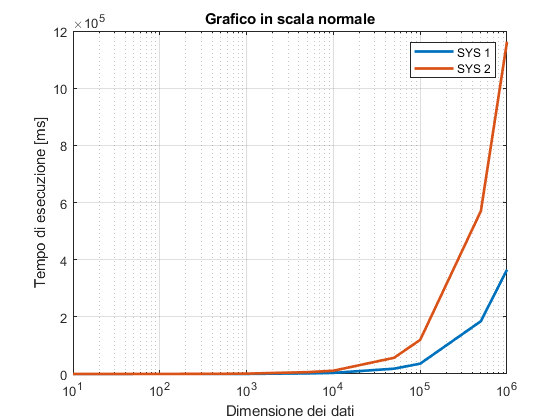
\includegraphics[width=0.8\textwidth]{img/hw0/grafico_naturale.png}
	\caption{\textit{Confronto andamento tempi di risposta sys1 e sys2}}
\end{figure}
\begin{figure}[H]
	\centering
	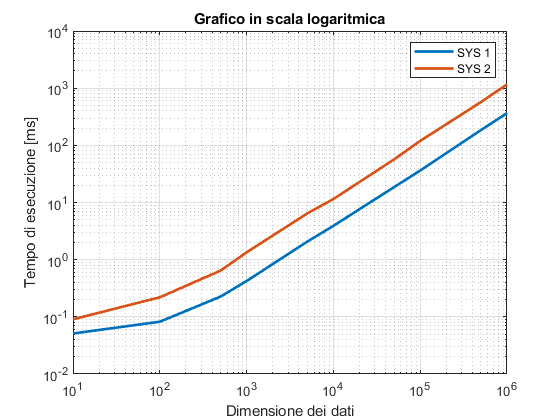
\includegraphics[width=0.8\textwidth]{img/hw0/grafico_log.png}
	\caption{\textit{Confronto andamento tempi di risposta - scala logaritmica}}
\end{figure}
Quindi il primo sistema è con evidenza quello più performante. Le differenze si percepiscono a vista d'occhio già a partire da \textit{N > $10^4$}.